%_____________________________________________________________________________________________ 
% LATEX Template: Department of Comp/IT BTech Project Reports
% Main Report
% Sun Apr 1 20:40:00 IST 2011
% 
%_____________________________________________________________________________________________ 

\documentclass[a4paper,12pt,onecolumn]{report}
%_____________________________________________________________________________________________ 
% Inclusion of Required Packages
%_____________________________________________________________________________________________ 
\usepackage[dvips]{graphics}
\usepackage{color}
\usepackage{epsfig}
\usepackage{longtable}
\usepackage{enumitem}
%_____________________________________________________________________________________________ 
% Page Layout
%_____________________________________________________________________________________________

 \usepackage[left=2.5cm,top=2cm,right=2cm,bottom=2cm,bindingoffset=0.5cm]{geometry}

%\usepackage{geometry}
%\geometry{a4paper,left=35mm,right=20mm,top=20mm,bottom=20mm}
\setlength{\textwidth}{6.5in}
\setlength{\textheight}{10in}
\setlength{\topmargin}{0.0in}
\setlength{\oddsidemargin}{0.0in}			% Customisable
\setlength{\headheight}{0.0in}
\setlength{\headsep}{0.0in}
\setlength{\topskip}{0.0in}
%_____________________________________________________________________________________________ 
% Font Definition
%_____________________________________________________________________________________________ 
\fontencoding{T1}		% Font specification : Times New Roman, Bold, Normal, 18
\fontfamily{cmr}		% Roman
\fontseries{m}			% Medium
\fontshape{n}			% Upright
\fontsize{14pt}{5}		
\linespread{1.5}		% Vertical spacing between lines
\selectfont			% Select the specified font
%_____________________________________________________________________________________________ 
% Main report starts here
%_____________________________________________________________________________________________ 
%\def\LT@c@ption#1[#2]#3{%
%  \LT@makecaption#1\fnum@table{#3}%
%  \def\@tempa{#2}%
%  \ifx\@tempa\@empty\else
%     {\let\\\space
%     \addcontentsline{lot}{table}{\protect\numberline{\thetable}{#2}}}%
%  \fi}


%\makeatletter
%\def\LT@c@ption#1[#2]#3{%
%  \LT@makecaption#1\fnum@table{#3}%
%  \def\@tempa{#2}%
%  \ifx\@tempa\@empty\else
%     {\let\\\space
%     \addcontentsline{lot}{table}{\protect\numberline{Table \thetable.}{#2}}}%
%  \fi}
%\makeatother


\setlength\LTcapwidth{\textwidth}

\makeatletter
  \def\LT@makecaption#1#2#3{%
    \LT@mcol\LT@cols c{\hbox to\z@{\hss\parbox[t]\LTcapwidth{%
    \vskip\abovecaptionskip
    \centering{
      \sbox\@tempboxa{#1{#2 }#3}%
      \ifdim\wd\@tempboxa>\hsize
        #1{#2. }#3%
      \else
        \hbox to\hsize{\hfil\box\@tempboxa\hfil}%
      \fi
      \endgraf\vskip\baselineskip}}%
    \hss}}}
\makeatother

\makeatletter
  \def\LT@c@ption#1[#2]#3{%
    \LT@makecaption#1\fnum@table{#3}%
    \def\@tempa{#2}%
    \ifx\@tempa\@empty\else
    {\let\\\space
      \addcontentsline{lot}{table}{\protect\numberline{\thetable}{\ignorespaces #2}\vspace\baselineskip}%
    }%
    \fi
  }
\makeatother

\begin{document}	% Start of Report
%_____________________________________________________________________________________________ 
%\pagestyle{empty}
%_____________________________________________________________________________________________ 
% Title page: Specifies a custom-made title page
%_____________________________________________________________________________________________ 
\DeclareGraphicsExtensions{.png, .ps}
\begin{titlepage}
\begin{center}
\LARGE{\bf{QUIZ GENERATION CHATBOT\\}}	% LARGE = 17.28
%\vspace{10pt}
\Large{\bf{A Project Report\\}}		% Large = 14.40
\Large{\em{Submitted by\\}}
\begin{table}[htbp]
	\begin{center}
	\begin{tabular}{ l c c l }
	\Large\bf{Vivek R. Bhave} & & & \Large\bf{111508015} \\[0.3cm] 
	\Large\bf{Shreyansh R. Gopawar} & & & \Large\bf{111508073} \\[0.3cm]
	\Large\bf{Aditya D. Neralkar} & & & \Large\bf{111508076} \\
	\end{tabular}
	\end{center}
	\end{table}
\Large{\em{in partial fulfillment for the award of the degree\\ \vspace{1.5pt}of\\}}
\LARGE{\bf{Information Technology\\}}% Mention only appropriate degree.
%\vspace{10pt}
%names of advisors
\Large{Under the guidance of\\ }
\Large{\bf{Dr. Y. V. Haribhakta}\\}
\Large{College of Engineering, Pune\\}
%\vspace{8pt}
% this is applicable only if you have a company based project
%\large{\bf{AND}\\}	% Case changed from full uppercase. Different from doc template. Looks better
%\vspace{10pt}
%\Large{\bf{Mr. Amit Kumar Singh}\\}
%\Large{Hindustan Naturals, Inc.\\}
%\vspace{5pt}
%coep logo added
%\begin{figure}[h]
%\centering
%
\includegraphics[width=3cm,height=3cm]{coeplogo.eps}
%\end{figure}
\Large{\bf{DEPARTMENT OF COMPUTER ENGINEERING AND \\INFORMATION TECHNOLOGY,\\ 
COLLEGE OF ENGINEERING, PUNE-5}}
\vfill
\large{April, 2019}
\end{center}
\end{titlepage}

%\maketitle			% *Generate* the defined title. No definition - no gereration

%_____________________________________________________________________________________________ 
% LATEX Template: Department of Comp/IT BTech Project Reports
% Certificate Page
% Sun Mar 27 10:25:35 IST 2011
% 
% Note: UK English spellings used. 
%_____________________________________________________________________________________________ 
\thispagestyle{empty}
\linespread{2}
\begin{center}			% LARGE = 18
	\Large{\bf{DEPARTMENT OF COMPUTER ENGINEERING AND\\  INFORMATION TECHNOLOGY,\\ 
	       COLLEGE OF ENGINEERING, PUNE\\}}	
\end{center}

\vspace{20pt}			% Vertical space between dept name and ``certi''

\begin{center}
	\Large{\bf{CERTIFICATE\\}}
\end{center}

\vspace{20pt}

\linespread{1.5}			% Double spacing between lines
\selectfont
\large{
Certified that this project, titled ``QUIZ GENERATION''
has been successfully completed by \\ 
\begin{table}[htbp]
	\begin{center}
	\begin{tabular}{ l c c l }
	\Large\bf{Vivek R. Bhave} & & & \Large\bf{111508015} \\ [0.3cm]
	\Large\bf{Shreyansh R. Gopawar} & & & \Large\bf{111508073} \\ [0.3cm]
 	\Large\bf{Aditya D. Neralkar} & & & \Large\bf{111508076} \\ [0.3cm]
	\end{tabular}
	\end{center}
	\end{table} \\
and is approved for the partial fulfillment of the requirements for the degree of 
``B.Tech. Information Technology''.
}

%\vspace{60pt}

\begin{center}		% Horizontal spacing used to keep the signatures in columns at the ends of
			% lines

%SIGNATURE\hspace{\stretch{1}}SIGNATURE\\
\normalsize{\bf{Dr. Y. V. Haribhakta\hspace{\stretch{1}}Dr. V. Z. Attar\\
Project Guide\hspace{\stretch{1}}Head}\\
Department of Computer Engineering\hspace{\stretch{1}}Department of Computer Engineering\\
and Information Technology,\hspace{\stretch{1}}and Information Technology,\\
College of Engineering Pune,\hspace{\stretch{1}}College of Engineering Pune,\\
Shivajinagar, Pune - 5.\hspace{\stretch{1}}Shivajinagar, Pune - 5.}
\end{center}

		% Certificate page will come here. But its been typeset 
				% independently in certi.tex

%_____________________________________________________________________________________________ 
% LATEX Template: Department of Comp/IT BTech Project Reports
% Abstract of Report
% Sun Mar 27 10:34:00 IST 2011
%_____________________________________________________________________________________________ 
\newpage
%\begin{abstract}
%\addcontentsline{toc}{chapter}{Abstract}	% This makes sure abstract is included in contents.
\begin{center}
\Large \textbf{Abstract}
\end{center}
Asking questions to students has always been regarded as the best method to gauge the students learning capabilities. However, with the amount of content available, generating questions from domain experts, is a time consuming and expensive process. 

The task of Automatic Question Generation(AQG) aims to generate questions from a given piece of text which shall appropriately test the students mastery over the material. Plenty of research in the area of AQG has been done over the years. The current state of the art models use a bidirectional Long Short Term Memory encoder decoder system to solve the problem. The work presented here carries out an important task in one of the stages of the entire AQG system. 

The model we have designed takes the sentence to generate questions on, as input, and tags a few words of the sentence as answer words on which questions can be created. The model has been trained using the SQUAD and Google datasets. The model has been created using LSTM networks and other linear layer neural networks. 

As a part of the system, we also built a custom web crawler. On input of a specific topic to the crawler, it can find a list of relevant web pages and is also able to filter in the important content from those webpages. Thus, this is an end to end system, which can be used in many areas like education, quizzing, entertainment, etc. 
%\end{abstract}

%_____________________________________________________________________________________________ 
	% Absract: Independently typeset in file abstract.tex

\thispagestyle{empty}


\tableofcontents		% *Generate* the table of contents. No content - no table
				% LATEX needs to run 2-3 times over source to get this correct

\pagenumbering{roman}	% Lowercase roman numbering for prelim sections
\listoftables
\addcontentsline{toc}{chapter}{List of Tables}

\listoffigures
\addcontentsline{toc}{chapter}{List of Figures}

\chapter*{List of Symbols}
\addcontentsline{toc}{chapter}{List of Symbols}

\newpage
\pagenumbering{arabic}	% Change to Arabic numbers for main chapters.

%_____________________________________________________________________________________________ 
% LATEX Template: Department of Comp/IT BTech Project Reports
% Sample Chapter
% Sun Mar 27 10:25:35 IST 2011
%
% Note: Itemization, enumeration and other things not shown. A sample figure is included.
%_____________________________________________________________________________________________ 

\chapter{Introduction}

\section{Importance of Automatic Question Generation (AGS) Systems}

Gauging a student’s knowledge over a certain topic is one of the fundamental
problems in education systems. Quizzing students has long been accepted as one
of the best techniques to solve the problem. Studies conducted over the last
several decades have found that providing students with frequent and good number
of quiz questions leads to better understanding of the topics, than spending an
equal amount of time studying notes or textbooks. Quizzes can be used at several
places in the education domain. It can be used in MOOC’s to test if a student
has  grasped the concept properly, they can be used as standalone tests in
universities, or they can also be used as practice by students to discern their
command over the subject. 

However, with the volume of information available, generating questions from
domain experts is an expensive and time consuming process. The task of Automatic
Question Generation (AQG), in the field of Natural Language Processing, aims to
generate questions from a given text, such that students are appropriately
tested on their mastery over the subject.

\section{Neural Networks}

A neural network is an interconnected collections of neurons. The connections
between the neurons are modelled as weights and the final value that the neuron
stores is the weighted summation of all the inputs. A neural network consists of
an input layer, an output layer and multiple hidden layers.

\begin{figure}
	\caption{Basic Neural Network Diagram}
	\centering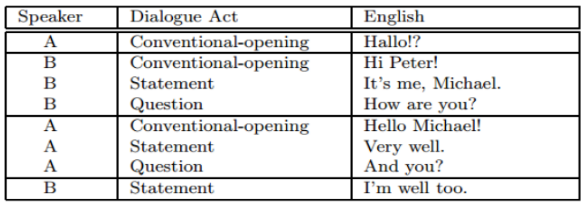
\includegraphics[width=10cm]{1.png}
\end{figure}

\section{Recurrent Neural Networks (RNN)}

Recurrent neural network is a type of artificial neural network. The problem of
remembering previous inputs to the network was solved by recurrent neural
networks with the help of hidden layers. Because of their internal memory, RNN
is able to remember important things about the input, which allows them to make
precise predictions about what’s coming next. This is why they are preferred
algorithm for sequential data. Sequential data is just ordered data where
related things follow each other.

\begin{figure}
	\caption{Recurrent vs Feed-forward Neural Network}
	\centering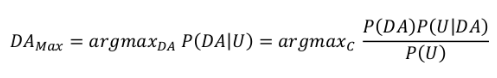
\includegraphics[width=10cm]{2.png}
\end{figure}

Unlike the normal feedforward neural networks, recurrent neural networks feed
the output of previous step to the current step. This helps the network to
memorise the previous inputs. So basically RNN cycles through the information,
i.e. when taking a decision it takes into consideration the current input as
well as whatever it learned from the previous output. For example, consider the
word ‘Teacher’, till the point a feed forward neural network reaches ‘c’ it
forgets about ‘t’, ‘e’ and ‘a’. A RNN remembers exactly that. Recurrent Neural
Network adds immediate past to the present. This is important since past data
contains information about what is coming next. 

RNN applies weight to current and also previous input and they tweak their
weights through gradient descent and backpropagation through time. Gradient
Descent is an algorithm that is used to iteratively minimize a given function.
Backpropagation Through Time (BPTT) is basically just a fancy buzz word for
doing Backpropagation on an unrolled Recurrent Neural Network. Unrolling is a
visualization and conceptual tool, which helps you to understand what’s going on
within the network. RNN can be viewed as a sequence of Neural Networks that is
trained one after another with backpropagation.

\begin{figure}
	\caption{Structure of a Neuron}
	\centering
\includegraphics[width=10cm]{3.png}
\end{figure}

The above diagram shows the RNN being unrolled after the equal sign. The
different timesteps are visualized and information gets passed from one timestep
to the next. Within BPTT the error is back-propagated from the last to the first
timestep, while unrolling all the timesteps. This allows calculating the error
for each timestep, which allows updating the weights.

\subsection{Problems with RNN}

\begin{enumerate}[align=left]

	\item Training RNNs is a difficult task.

	\item \textbf{Exploding gradient problem :} Exploding gradient is when
		the algorithm assigns a stupidly high importance to the weights,
		without much reason. But fortunately, this problem can be easily
		solved if you truncate or squash the gradients.

	\item \textbf{Vanishing gradient problem :} Vanishing gradient is when
		the values of a gradient are too small and the model stops
		learning or takes way too long because of that. This problem is
		solved by the concept of LSTM.

\end{enumerate}

\section{Long Short Term Memory}

Long Short Term Memory (LSTM) is an artificial recurrent neural network.
Consider LSTM as an extension to the recurrent neural network, which basically
extends its memory. Therefore they are capable of learning things that have very
large time lags between them. LSTM can remember this because they contain their
information in a memory, that is much like the memory of a computer because the
LSTM can read, write and delete information from its memory.

The memory in LSTM are gated cells. Gated cell means that he cell decides
whether or not to store or delete information based on the importance it assigns
to the information. The importance assigning takes place through weights which
are learned through the algorithm.

\begin{figure}
	\caption{Structure of a Basic LSTM node}
	\centering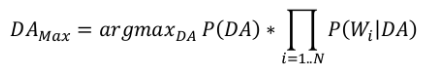
\includegraphics[width=10cm]{4.png}
\end{figure}

A basic LSTM node consists of input gate, output gate and forget gate. The input
gate decides whether or not to let new input in. The forget gate deletes the
information because it is not important. The output gate impacts the output at
the current time step. The gates in a LSTM are analog, in the form of sigmoids,
meaning that they range from 0 to 1. The fact that they are analog, enables them
to do backpropagation with it.

The problem of vanishing gradients which is very common in recurrent neural
networks is solved by LSTM as it keeps the gradient steep enough and therefore
the training short and the accuracy high.
	% Add each chapter here in this fashion.
				% No need to write all font and page specs in the chapter
				% files. There only typesetting tags are required.
%_____________________________________________________________________________________________ 
% LATEX Template: Department of Comp/IT BTech Project Reports
% Sample Chapter
% Sun Mar 27 10:25:35 IST 2011
%
% Note: Itemization, enumeration and other things not shown. A sample table is included.
%_____________________________________________________________________________________________ 

\chapter{Literature Survey}

\begin{enumerate}[align=left]

	\item \textbf{Computational Intelligence Framework for Automatic Quiz
		Question Generation}
		
		The model described in this paper, uses a rule based approach
		and is able to generate three types of questions, namely, Fill
		in the Blank, True/False, and “Wh” Questions. The training phase
		of this algorithm involves, detecting topically important
		sentences, NER and POS Tagging, sanitizing the input sentence
		and then constructing a tree for further processing of each type
		of question.  For Fill in the Blank, it gives weight to each
		word involved and marks important words for setting up blanks.
		Thr true or false sentence involves identifying modal verbs, and
		also factual type of sentences and further rule based
		processing. For “Wh” questions, patterns identified during the
		training phase are matched, and used to generate questions. 

\item \textbf{Automatic Question Generation System}
	
	This is a traditional supervised learning approach and the model can be
		broken down into a sequence of processes.  The text input is
		stemmed to get the meaning of each word and then passed to the
		Phrase Mapper. Then the key phrases are extracted using pre
		trained documents and the document is summarized. In the end,
		Nouns are filtered in, on which questions can be generated. 

\item \textbf{Automatic Question Generation for Intelligent Tutoring Systems}
	
	This system generates only Multiple Choice Questions, and has been
		trained on Wikipedia articles. The wikipedia articles are
		processed and unigrams, bigrams are extracted. The keywords from
		them are then extracted and their weights using the TF IDF
		weighting scheme are calculated. Using the above distractors can
		be generated. Whenever a query is fired to generate questions
		on, the wikipedia articles of the keyword is taken up, and rule
		based methods are applied to the sentences to create questions
		and presented to the users including the distractors as other
		viable options. 

\item \textbf{Automatic Question Generation from Children’s Stories for
	Companion Chatbot}
		
This paper was specifically targeted for generating questions from children’s
		stories, and was trained and tested on much lesser data than
		others. The model is said to work in two parts, that is one for
		question generation and the other for ranking of the questions.
		The model uses the part of speech tags and dependency parsing
		algorithms along with pre trained language rules for the
		question generation phase. For ranking of the questions, the
		model uses logistic regression to determine the acceptability
		probability of the question. 

\item \textbf{Deep Guessing}
	
	Generating Meaningful Personalized Quizzes on Historical Topics by
		Introducing Wikicategories in Doc2Vec: The aim of this model is
		to load all of the wikipedia articles, classify them into
		categories, and use the knowledge from the above, for generation
		of distractors in multiple choice questions. The model works on
		a novel idea of creation of paragraph vectors, whose advantage
		is that they are trained from unlabeled data and thus can work
		well for tasks which do not have enough labelled datasets. After
		the score of wiki categories is obtained, thresholds are decided
		to classify the records into categories and thus, are eventually
		used for the creation of meaningful options in the questions
		generated. 

\item \textbf{Automatic question generation on the basis of the discourse
	connectives}
	
	This problem of question generation has been divided into two modules in
	this paper.  The first part is that of Content selection and the next
	that of Question formation. The Content selection phase consists of
	recognizing the part in text that is relevant and important to generate
	questions on. The second phase of Question formation includes several
	subtasks like Word Sense disambiguation of the discourse connectives
	then the Identification of the type of question to be created and
	eventually applying syntactic transformations on the context. The paper
	mainly takes into consideration the seven main discourse connectives -
	although, as a result, because, for example for instance and since.
	Using the output generated so far, the type of question gets decided and
	then the question can be formed. 

\item \textbf{Semantic Based Automatic Question Generation}
	
	The paper explains a system that applies two fundamental Natural
	Language Processing concepts namely Semantic Role Labeling and Named
	Entity Recognizer technique. These tasks are used to convert the
	inputted sentence to semantic pattern. The model described in the paper
	has developed a system which has identified patterns for each type of
	question. The question types under consideration here are all of the
	‘Wh’-questions - who, when, why, where, what.  The system for
	classification uses learning, storage memory, feature extraction, and
	associative Retrieval.  

The sentence given as input will be first parsed using Named Entity Recognition
and SRL technique. The output of these two algorithms has a direct correlation
with the exact question type to be created. Thus after the question type
identification, the question pattern is known using the pretrained rules. 

\item \textbf{Automatic Multiple Choice Question Generation System for Semantic
	Attributes Using String Similarity Measures}
	
	The paper has described a model which first selects a factual sentence
	and an important word to generate questions on from the text given as
	input. This selection is done on the basis of the semantic labels and
	named entities in the sentence. Then for actually generating a question
	the SRL and NER tag is used, which directly helps in finding out the
	type of question. 

Then the model focuses on finding distractors i.e. the incorrect options of a
question. For this task  different similarity measure between sentences of the
data set is taken into account. Eventually, when a question is generated, the
measures of similarity between the actual question and the sentences of the
input text is considered and sorted. The top three sentences obtained from the
above procedure, are considered for finding a relevant important word to the
question generated which are eventually used as distractors. 

\end{enumerate}

\begin{center}
	\begin{longtable}{| p{0.6cm} | p{2.3cm} | p{4cm} | p{2cm} | p{5cm} |}
		\caption{Comparison Table}\\
		\hline
		{\textbf{Sr No.}} & {\textbf{Algorithm}} & {\textbf{Methodology}} &
		{\textbf{Type of Question}} & {\textbf{Evaluation of Result}}\\[2ex]
		\hline
		1. &
		Computationally Intelligent Techniques &
		Rule Based Approach - Training for patterns and then generate &
		Fill in the Blanks, True/False, “Wh” questions & 
		Manual checking for finding difference between Automatic Questions and Domain Experts - users found difference 
		\\[1ex]
		\hline

		2. &
		Automatic Question Generation System &
		Series of pre processes like stemming, summarize, noun extract, and then rule based question generation &
		All “Wh” questions along with type like - Person, Definition, Procedure, Consequence, etc &
		Compression and Omission Ration considered - acceptable results
		\\[1ex]
		\hline
		3. &
		AQG for Intelligent Tutoring Systems &
		Keywords from Wikipedia and then TF-IDF, then rule based &
		MCQ’s alongwith distractors &
		Manual evaluation with domain expert
		\\[1ex]
		\hline
		4. &
		AQG from Children’s Stories for Companion Chatbot  &
		POS Tagger, Dependency Parsing and Logistic Regression &
		Only “Wh” questions &
		Manual evaluation with over 50\% acceptance		
		\\[1ex]
		\hline
		5. &
		Deep Guessing: Quizzes on Historical Topics by Wikicategories in Doc2Vec:  &
		Generating paragraph vectors from wikipedia articles, categorization for distractors &
		MCQ Questions with distractors &
		Manual evaluation of 45 MCQ’s \\[1ex]
		\hline
		6. &
		AQG on the basis of the discourse connectives &
		Content selection and Question formation &
		Question generation like Why, when, where, in which &
		Manually evaluated for semantic and syntactic soundness of question by two evaluator 
		\\[1ex]
		\hline
		7. &
		Semantic based AQG &
		Feature Extraction using NER, SRL, Sentence pattern finding and  get question type pattern &
		Only “Wh” questions &
		Manual evaluation with small dataset, About 87\% accuracy		
		\\[1ex]
		\hline
		8. &
		AQG System for Semantic Attributes Using String Similarity Measures &
		Extracting sentence, check viability by similarity of sentences and select top three sentences &
		Only “MCQ” type questions &
		Manual evaluation with 75\% success. 
		\\[1ex]
		\hline
	\end{longtable}
\end{center}


%\begin{table}[H]		% Table
%\begin{center}		
%\begin{tabular}{ | c | c | }	% Format	
%\hline
%\multicolumn{2}{|c|}{Table 1: Test Century Records }\\
%\hline
%\bf{Batsman} & \bf{Test Centuries}\\ \hline
%Sachin & 51 \\ \hline
%Kallis & 40 \\ \hline
%Ponting & 39 \\ \hline
%Lara, Gavaskar & 34\\ 
%\hline
%\end{tabular}
%\caption{A simple table: Test centuries}	% This will appear in List of Tables
%\label{table1}
%\end{center}
%\end{table}

%_____________________________________________________________________________________________ 

		
\chapter{Problem Statement} 

The problem of question generation, is currently solved by domain experts, who
create questions over text or topics by their intuition or knowledge. Automatic
Question Generation can solve this laborious, time consuming task quite
efficiently and much higher accuracy. Such an automatic question generation
system can have applications in multiple domains. 

\section{Motivation} 

The main motivation of designing an Automatic Question Generation System, was
contribution in the education domain. Generating quiz questions can be of utmost
importance for teachers to ensure that students are able to understand the
material in class, and at the same time, can become an easy way out for students
to find out their preparedness over the subject, studying independently. 

\section{Objectives}

The objective of the project is to take a topic as input from the user, and
generate a set of questions related to the topic to present to the user. The
questions generated through such a system, should be similar to questions
generated by a domain expert. Also the difficulty level of the questions, should
be such that they can appropriately test the knowledge of the user. 

		

\appendix
\chapter{Algorithm}
\chapter{Flow Chart for Making Popcorn}

\bibliographystyle{plain}  % You can change the style of writing bibliography.
\bibliography{coep_compit_report} % Instead of a .bib file, you can just write it in 
				  % a text file with \bibitem entries.
%_____________________________________________________________________________________________ 
\end{document}			% End of Report

